\section{Filter-Functions}

\textbf{Pass band:} Frequency range where the signal passes through the filter.\\
\textbf{Stop band:} Frequency range where the signal is attenuated by the filter.\\
\textbf{Cut-off frequency:} Frequency where the signal is attenuated by 3 dB.\\
\textbf{Attenuation:} The decrease in signal strength.\\
\textbf{Ripple:} The variation in the pass band.\\
\textbf{Form factor:} The ratio between the stop band and the pass band.\\
\textbf{Group delay:} The time delay of the filter.\\
\textbf{Phase delay:} The phase shift of the filter.

\subsection{Electronic filters}
\textbf{Low-pass filter:} Ideally only allows low angle frequencies ($\omega<\omega_{a}$)
\begin{center}
  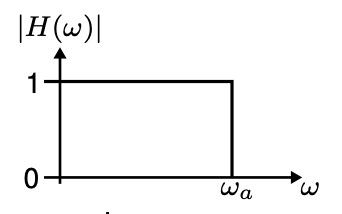
\includegraphics[width=0.25\textwidth]{Images/Lowpass.png}
\end{center}

\textbf{High-pass filter:} Ideally only high angle frequencies ($\omega>\omega_{a}$)
\begin{center}
  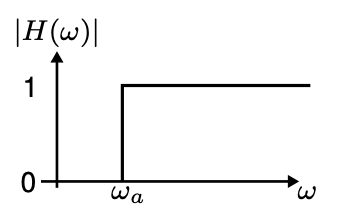
\includegraphics[width=0.25\textwidth]{Images/Highpass.png}
\end{center}

\textbf{Band-pass filter:} Ideally only certain range of angle frequencies ($\omega_{1}<\omega>\omega_{2}$) 
\begin{center}
  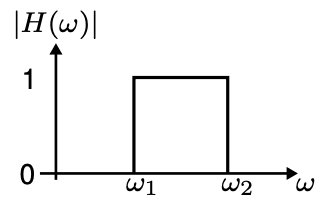
\includegraphics[width=0.25\textwidth]{Images/Bandpass.png}
\end{center}

\textbf{Band-stop filter:} Ideally filters out a certain range of angle frequencies ($\omega_{1}>\omega<\omega_{2}$) 
\begin{center}
  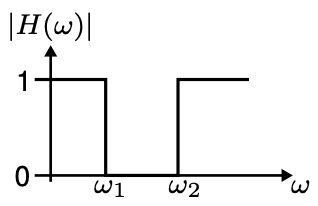
\includegraphics[width=0.25\textwidth]{Images/Bandstop.png}
\end{center}

\subsection{Filter specification}
Specifications for a low-pass filter could be:
\begin{enumerate}
  \item A cut-off frequency $\omega_{a}$ that specifies the upper limit of the passband.
  \item A stopband frequency $\omega_{s}$ at which a stopband attenuation As is specified. 
  \item Information about permissible gain variation in the passband.
\end{enumerate}


\subsection{Group delay}
Measures time for the filter and often depend on frequency $\omega$.
$$T_{g}=-\frac{ d\phi(\omega) }{ d\omega } $$
where $\phi(\omega)$ is the angle of the filter.

The phase characteristic of a filter also affects the input-output behavior of a filter. If pulse overshoot or damped oscillation (ringing) is to be avoided, the filter must have a constant group delay, $T_{g}$.

\subsection{Filter transfer functions}
In practice, the ideal filters cannot be realized, but can be approximated using various filter function types.

These are all-pole filters (Only poles, no zeros)
When selecting the filter function for a given application, we are interested in the following characteristics:
\begin{enumerate}
  \item Constant gain in passband.
  \item High attenuation after cut-off frequency.
  \item Linear phase.
\end{enumerate}

\begin{center}
  \includegraphics[width=\textwidth]{Images/Filter-Transform.png} 
\end{center}

\subsubsection{Butterworth}
$$|H(j\omega)|^2=\frac{1}{1+(\frac{\omega}{\omega_{a}})^{2N}}$$
where $\omega_{a}$ is the cut-off frequency [rad/s]

All poles for $H(j\omega)$ lie in the left half-plane on a circle with radius $\omega_{a}$ and centre at the origin.

A Butterworth filter has the following characteristics:
\begin{enumerate}
  \item Optimal in terms of constant gain in the passband.
  \item Has 3 dB attenuation at the cut-off frequency and then the filter gain drops rapidly by 20 dB/dec. (dec is when the power of 10 changes by 1)
  \item The phase of the filter is not constant in the passband, which causes ringing at the step input.
\end{enumerate}
All pole pairs of a Butterworth filter have a natural frequency $\omega_{n}$, which is equal to the cut-off frequency $\omega_a$.

Construction tables: Page 169 (Digital Signal Behandling: Erik Hüche)\\
Amplitude characteristics to determine order: Page 161 (Digital Signal Behandling: Erik Hüche)


\subsubsection{Chebyshev}
$$|H(\omega)|^2=\frac{1}{1+e^{ 2 }T_{N}^2(\omega-\omega_{a})}$$
where $T_{N}(\omega)$ is Chebyshev polynomial of degree N given by
$$T_{N}(\omega)=\left\{ \begin{array}{cl}
\cos(N\cdot \cos^{-1}(\omega)) & : \ |\omega| \leq 0 \\
\cosh(N\cdot \cosh^{-1}(\omega)) & : \ |\omega| > 0
\end{array} \right.$$

The size of the passband ripple $\delta$ in dB is given by $\epsilon$
$$\delta=10\cdot \log(\epsilon^2+1)$$
A Chebyshev filter has the following characteristics 
\begin{enumerate}
  \item Has varying gain in the passband - the size of the passband ripple can be freely selected. 
  \item The gain decreases rapidly around the cut-off frequency. 
  \item The phase of the filter is not constant in the passband, which causes ringing at the step input.
\end{enumerate}
The DC gain of a Chebyshev low-pass filter is not the maximum gain of the filter if the pole count is even.

Construction tables: Page 170 (Digital Signal Behandling: Erik Hüche)\\
Amplitude characteristics to determine order: Page 162 (Digital Signal Behandling: Erik Hüche)

\subsubsection{Bessel}
The transfer function for an Nth order Bessel filter is
$$H_{N}(s)=\frac{b_{0}}{s^N+b_{N-1} s^{N-1}+\cdots +b_{1}s+b_{0}} $$
where
$$b_{k}=\frac{(2N-k)!}{2^{N-k}k!(N-k)!}$$
A Bessel filter has the following properties:
\begin{enumerate}
  \item Does not have ripple in the passband, but the amplitude is not as constant as a Butterworth filter. 
  \item Has attenuation that is very smooth. The amplitude characteristic of the filter is like that of the first order filter for the first 6 dB of attenuation regardless of the number of poles. 
  \item The phase is almost linear with frequency within the passband.
\end{enumerate}

Construction tables: Page 173 (Digital Signal Behandling: Erik Hüche)\\
Amplitude characteristics to determine order: Page 163 (Digital Signal Behandling: Erik Hüche)

\subsubsection{The filter's order number}
The order number of filters can be found by reading the amplitude characteristic of a given filter function and comparing it to the attenuation requirements at the stopband frequency. 
$$Y=20\log\left( \frac{A}{A_{\text{ max }}} \right)$$
Frequency normalised (form factor)
$$X=\frac{\omega}{\omega_{a}}$$


\subsection{Filter transformers}
\subsubsection{Low pass to high pass transformation}
High-pass filters can be designed from normalised prototype low-pass filters based on the following specification:
\begin{itemize}
  \item The filter function (Bessel, Butterworth, Chebyshev) 
  \item The filter cut-off frequency $\omega_{a}$
  \item The filter stopband frequency $\omega_{s}$
  \item The filter stopband attenuation $A_{s}$ at the stopband frequency $\omega_{s}$
\end{itemize}

\begin{center}
  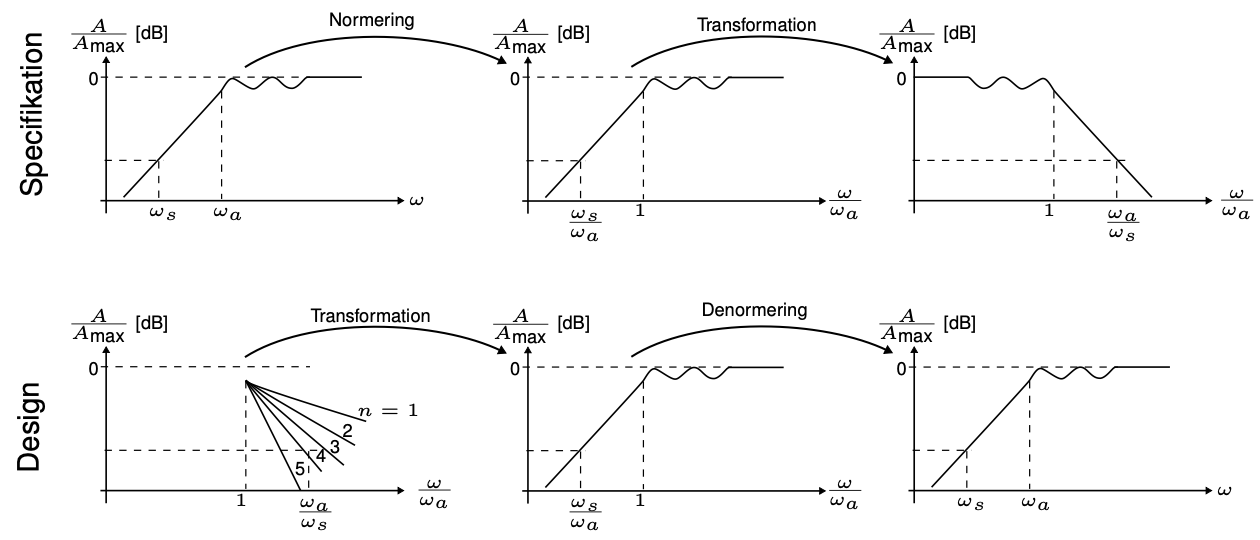
\includegraphics[width=\textwidth]{Images/LP-to-HP.png} 
\end{center}
A low-pass filter can be transformed into a high-pass filter by:
$$H_{\text{hp}}(s)=H_{\text{lp}}(\bar{s})|_{\bar{s}=\frac{1}{s}}$$

Process: Low pass to high pass transformation
\begin{enumerate}
  \item Find the stopband frequency for the normalized low-pass filter (used for the design):$$\frac{\omega_{a}}{\omega_{s}}=\frac{f_{a}}{f_{s}}$$
  \item Filter order selection based on amplitude characteristics for lowpass filters.
  \item The transfer function of the normalized low-pass filter is transformed to the transfer function of the normalized high-pass filter by replacing $s$ with $\frac{1}{s}$
  \item The transfer function of the denormalized high-pass filter is found by replacing $s$ with $\frac{s}{\omega_{a}}$
\end{enumerate}


\subsubsection{Low pass to bandpass transformation}
Bandpass filters can be designed from normalized prototype low-pass filters based on the following specification
\begin{itemize}
  \item The filter function (Bessel, Butterworth, Chebyshev) 
  \item The filter center frequency $\omega_{s}$
  \item The passband bandwidth $\Delta \omega _a$
  \item Stopband bandwidth $\Delta \omega _s$
  \item Filter stopband attenuation $A_{s}$
\end{itemize}

\begin{center}
  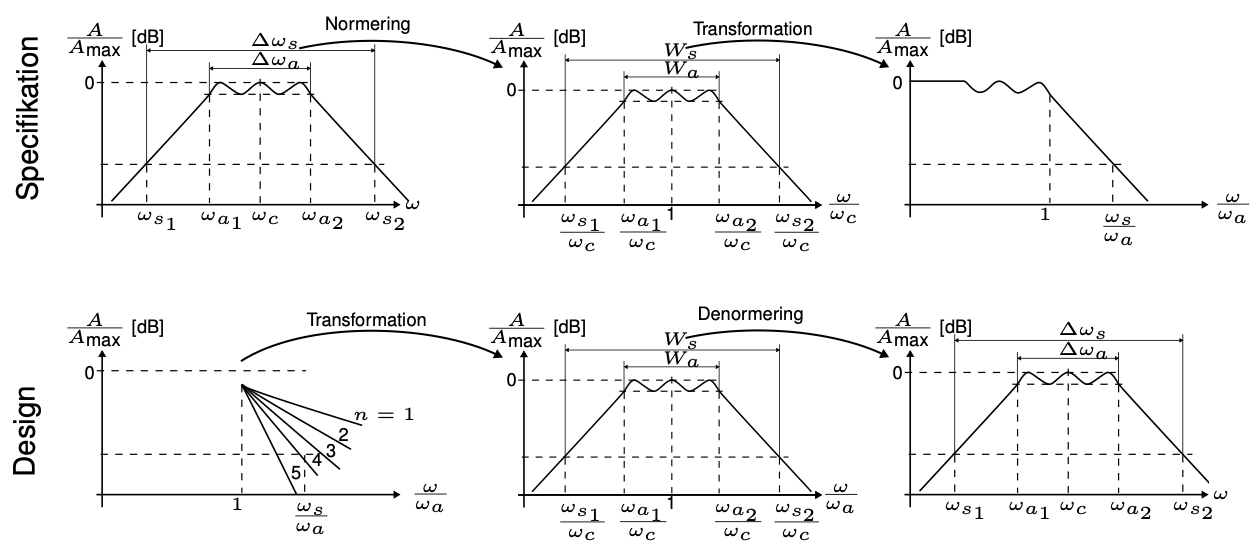
\includegraphics[width=\textwidth]{Images/LP-to-BP.png} 
\end{center}
A low-pass filter can be transformed into a bandpass filter by
$$H_{\text{bp}}(s)=H_{\text{lp}}(\bar{s})|_{\bar{s}=\frac{1}{W_{a}}\left( s+\frac{1}{s} \right)}$$

To design the filter, the bandpass filter is normalised, i.e. the normalised stopband width and the normalised passband width are calculated as:
$$W_{a}=\frac{\Delta f_{a}}{f_{c}}$$
$$W_{s}=\frac{\Delta f_{s}}{f_{c}}$$
$$\omega_c=\sqrt{\omega_{a_1}\cdot\omega_{a_1}}$$
If $\omega_c$ and $\Delta\omega_a$ is known:
$$\omega_{a_1}=\sqrt{\frac{(\Delta \omega_a)^2}{4}+\omega_c^2}-\frac{\Delta\omega_a}{2}$$
$$\omega_{a_2}=\sqrt{\frac{(\Delta \omega_a)^2}{4}+\omega_c^2}+\frac{\Delta\omega_a}{2}$$
These can also be used with $\omega_s$

The form factor for bandpass filter:
$$F=\frac{\Delta f_{s}}{\Delta f_{a}}=\frac{W_{s}}{W_{a}}$$


Process: Low pass to bandpass transformation
\begin{enumerate}
  \item To design the filter, the bandpass filter is normalized, i.e. the normalized stopband width and the normalized passband width are calculated.
  \item The form factor is found.
  \item Filter order selection based on amplitude characteristics for lowpass filters.
  \item The normalised filter is found by replacing $s$ with $\frac{1}{W_{a}} \left( s + \frac{1}{s} \right)$ in the low-pass filter.
  \item The denormalized bandpass filter is found by replacing $s$ in the normalized bandpass filter with $\frac{s}{\omega_{c}}$.
\end{enumerate}

\subsubsection{Low pass to bandstop transformation}
Bandstop filters can be designed from normalised prototype low-pass filters based on the following specification:
\begin{itemize}
  \item Filter function (Bessel, Butterworth, Chebyshev) 
  \item Filter centre frequency $\omega_{c}$ 
  \item Passband bandwidth $\Delta\omega_{c}$ 
  \item Stopband bandwidth $\Delta\omega_{s}$ 
  \item Filter stopband attenuation $A_{s}$
\end{itemize}

\begin{center}
  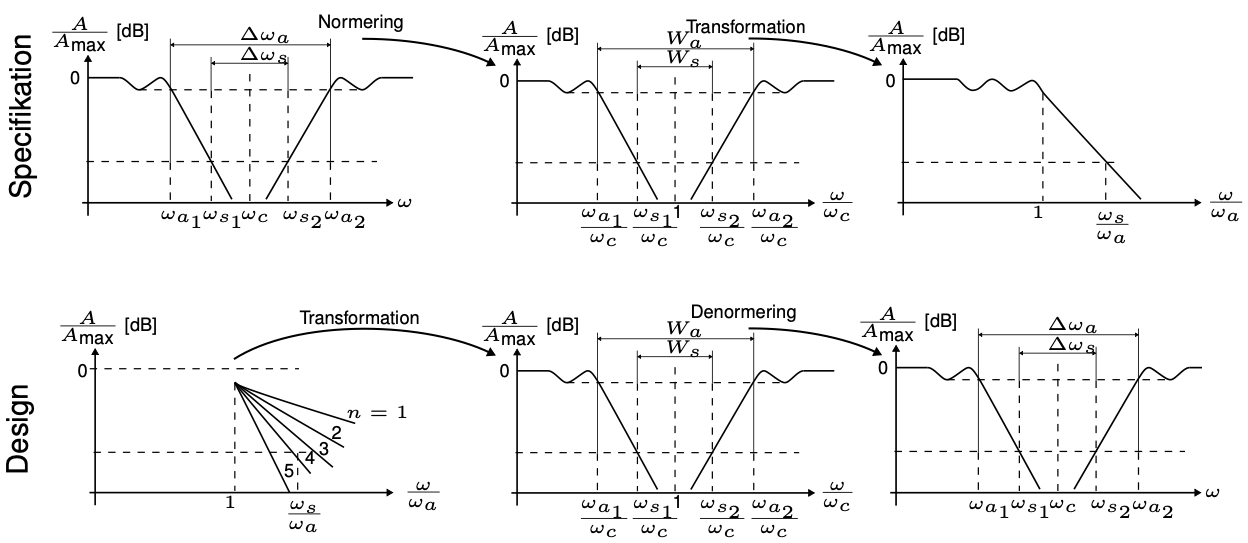
\includegraphics[width=\textwidth]{Images/LP-to-BS.png} 
\end{center}
A low-pass filter can be transformed into a bandstop filter by
$$H_{\text{bs}}(s)=H_{\text{lp}}(\bar{s})|_{\bar{s}=\frac{W_{a}}{s+\frac{1}{s}}}$$
and the form factor for bandstop filter:
$$F=\frac{\Delta f_{a}}{\Delta f_{s}}=\frac{W_{a}}{W_{s}}$$

Process: Low pass to bandstop transformation
\begin{enumerate}
  \item To design the filter, the bandstop filter is normalized, i.e. the normalized stopband width and the normalized passband width are calculated.
  \item The form factor is found.
  \item Filter order selection based on amplitude characteristics for lowpass filters.
  \item The normalised filter is found by replacing $s$ with $\frac{W_{a}}{s+\frac{1}{s}}$ in the low-pass filter.
  \item The denormalized bandpass filter is found by replacing $s$ in the normalized bandpass filter with $\frac{s}{\omega_{c}}$.
\end{enumerate}

\subsection{Examples}
\subsubsection{Example 1:}
